\documentclass[class=article , crop=false, titlepage, twoside, multi={itemize, figure, verbatim}, float=false]{standalone}

\usepackage{import} % Required for importing other .tex docs.  (import uses everything bw Begin and End Doc)
\usepackage{float} % Required for specifying the exact location of a figure or table
\usepackage{graphicx} % Required for including images
\usepackage{wrapfig}
\usepackage[pdftex,breaklinks,colorlinks=true,linkcolor=black,citecolor=blue,urlcolor=red,linktocpage=false,pagebackref=true,filecolor=magenta]{hyperref}%http://www.tug.org/applications/hyperref/manual.html#x1-100003.6
\usepackage{cite}
\usepackage[toc,title,page]{appendix}
\usepackage{pdfpages} % enables loading a pdf into the doc
\usepackage{makeidx}
\usepackage{glossaries} % must be after hyperref
\usepackage{blindtext}
\usepackage{enumitem}
%\usepackage{caption}

%\setlist[description]{leftmargin=\parindent,labelindent=\parindent}

%\renewcommand*{\bibname}{References} % renames the bibliography

\newcommand{\HRule}{\rule{\linewidth}{0.5mm}} % Command to make the lines in the title page

\graphicspath{{img/}{GIS_ChampionSection/img/}{awardsChapter/GIS_ChampionSection/img/}{brandPart/awardsChapter/GIS_ChampionSection/img/}{img/}{pairedProgSection/img/}{methodChapter/pairedProgSection/img/}{methodPart/methodChapter/pairedProgSection/img/}{documentationSection/img/}{methodChapter/documentationSection/img/}{methodPart/methodChapter/documentationSection/img/}{docStorageOrgSection/img/}{methodChapter/docStorageOrgSection/img/}{methodPart/methodChapter/docStorageOrgSection/img/}{QGisSection/img/}{toolsChapter/QGisSection/img/}{servicePart/toolsChapter/QGisSection/img/}{ESRISection/img/}{toolChapter/ESRISection/img/}{servicePart/toolChapter/ESRISection/img/}{../../../../source/}{../../source/}{servicePart/applicationsChapter/treasurerSection/img/}}

%\setlength\parindent{0pt} % eliminates indents


\def\titlename{Geodatabase Replicas\\ \medskip\large Managing Enterprise Geodatabase Replicas in ArcGIS}

\title{\HRule % Horizontal Line added
\\[.4cm] % space
\begin{figure}[H] % included image
\begin{center}	% centered horizontally
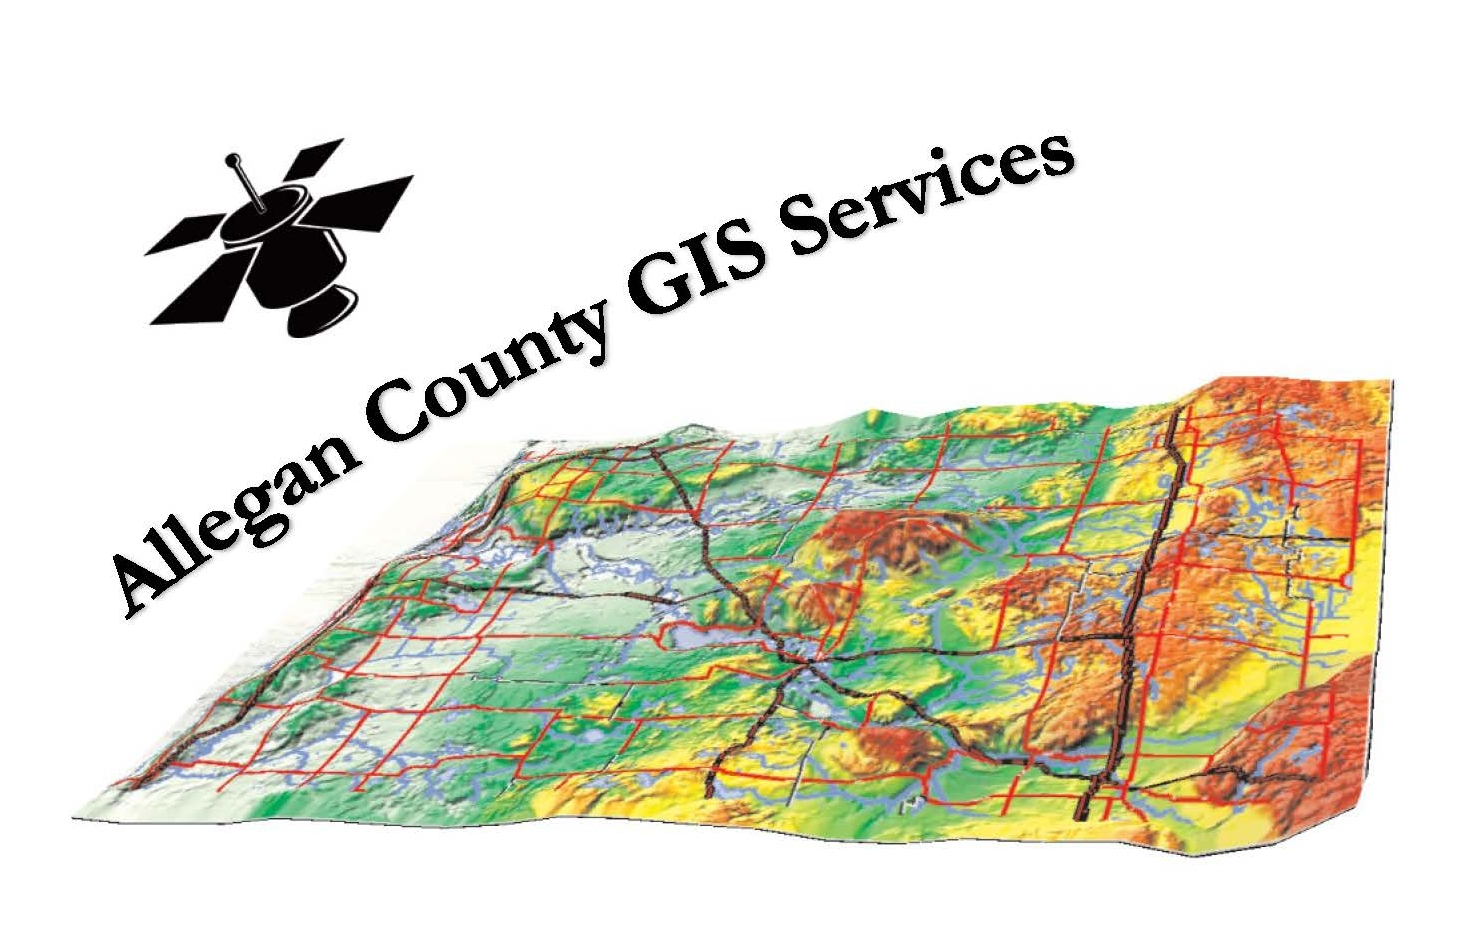
\includegraphics[scale=.45]{GIS_Logo_better.jpg}
\end{center}
\end{figure}
\Huge \bfseries \titlename \\ % Title text
\HRule \\[.4cm] % Horizontal Line added
\author{\Large Allegan County GIS \\\Large www.allegancounty.org/gis} % defines author
}  % inputs common title
\setcounter{tocdepth}{5}  % subparagraph and down
\begin{document}% document begins


\ifstandalone
%\frontmatter % turns off chapter numbering and uses roman numerals for page numbers
\maketitle % creates title page and blank page after title page
\tableofcontents % creates TOC and blank page
\clearpage
%\mainmatter % turns on chapter numbering, resets page numbering and uses arabic numerals for page numbers
\fi

\subsection{Managing Geodatabase Replicas}
\medskip 
\subsubsection[Adding A New Feature Class To A Replica]{\Large Adding A New Feature Class To A Replica}

Source:
\href{https://support.esri.com/en/technical-article/000010345}{https://support.esri.com/en/technical-article/000010345}

\paragraph[Summary]{Summary \texorpdfstring{\\}{}}
Currently, there is no out-of-the-box tool to add a feature class to an existing replica. With ArcGIS Desktop, one must either recreate the replica or if the workflow allows, replicate the new feature class as a separate replica.

A feature class or table can only be added to an existing replica (without recreating the replica) using ArcObjects code.

\paragraph[Steps]{Steps:\texorpdfstring{\\}{}}

The steps below outline how the recreate the replica using the Register Existing Data option in Desktop. These steps can be applied to both one-way and two-way replicas.


Synchronize the changes between parent and child replica geodatabases using the existing replica so that the data is identical in each database, then Unregister the replica in both geodatabases. For two-way replicas, ensure that changes are synchronized in both directions and there are no outstanding edits before unregistering the replica.
Create/import the new feature class into the parent geodatabase, and add the GlobalID.
Register the newly added data as versioned.
Copy and paste the new feature class to the child geodatabase using ArcCatalog. 
Note:
 that the GlobalIDs must have already been added to the feature class.

For two-way replica or one-way full model, register the newly added data in child geodatabase as versioned.
Using the parent geodatabase, add all the data that is to be replicated to a map in ArcMap.
Click the 'Create Replica' tool on the Distributed Geodatabase toolbar.
Select 'One way replica' or 'Two way replica' and click Next.
Select 'Register existing data only'.
Select the child geodatabase and specify a replica name.
Click Next and click Finish.
A new replica is created that includes the new data.
\end{document}